\documentclass[12pt,addpoints]{repaso}
\grado{2}
\nivel{Secundaria}
\cicloescolar{2023-2024}
\materia{Ciencias y Tecnología: Física}
\unidad{1}
\title{Repaso para el examen de la Unidad}
\aprendizajes{\scriptsize%
\item Describe problemas comunes de la vida cotidiana explicando cómo se procede para buscarles solución; conoce y caracteriza el pensamiento científico para plantearse y resolver problemas en la escuela y su cotidianidad.\\[-1.5em]
\item Identifica las unidades de medición que se ocupan en su entorno escolar, familiar y en su comunidad.\\[-1.5em]
\item Identifica cuáles son, cómo se definen y cuál es la simbología de las unidades básicas y derivadas del Sistema Internacional de Unidades.\\[-1.5em]
\item Indaga sobre los saberes y prácticas del uso de materiales y sus propiedades y características para construcción, vestimenta y artefactos de uso común.\\[-1.5em]
\item Relaciona e interpreta las teorías sobre estructura de la materia, a partir de los modelos atómicos y de partículas y los fenómenos que les dieron origen.\\[-1.5em]
\item Explora algunos avances recientes en la comprensión de la constitución de la materia y reconoce el proceso histórico de construcción de nuevas teorías.\\[-1.5em]
\item Experimenta e interpreta los modelos atómicos y de partículas al proponer hipótesis que expliquen los tres estados de la materia, sus propiedades físicas como la temperatura de fusión, ebullición, densidad, entre otros.\\[-1.5em]
\item Interpreta la temperatura y el equilibrio térmico con base en el modelo de partículas.\\[-1.5em]
}
\author{Melchor Pinto, J.C.}
\begin{document}
\INFO%
\begin{questions}
     \questionboxed[5]{Coloca los conceptos en el lugar que les corresponda en la imagen.\\

          \begin{center}
               \wordpill{Sublimación}
               \wordpill{Fusión}
               \wordpill{Ebullición}
               \wordpill{Sólido}
               \wordpill{Líquido}
               \wordpill{Gaseoso}
               \wordpill{Solidificación}
               \wordpill{Condensación}
               \wordpill{Deposición}
               \vspace*{1em}
               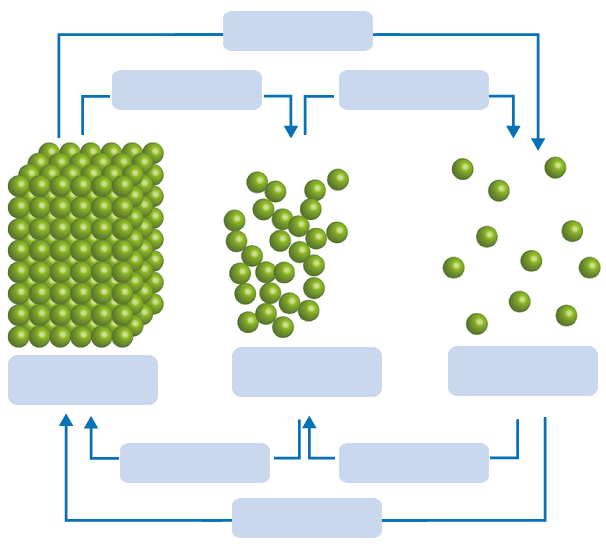
\includegraphics[width=.75\textwidth]{../images/SINFI_U2_AC47_IMG1.png}
          \end{center}
     }

     \questionboxed[5]{Elige la(s) respuesta(s). Pueden existir más de 2 respuestas correctas.
          \begin{multicols}{2}
               \begin{parts}
                    \part  Los conocimientos políticos se refieren a \dots

                    \begin{checkboxes}
                         \choice métodos para producir o transformar la naturaleza
                         \choice lo que la sociedad considera bueno o malo y necesario para la convivencia.
                         \choice los que se utilizan para obtener un bien material o resolver un problema real.
                         \CorrectChoice la organización y forma de gobierno de la sociedad.
                    \end{checkboxes}


                    \part Los conocimientos tradicionales son:

                    \begin{checkboxes}
                         \CorrectChoice transmitidos de generación en generación en una cultura y que les da identidad
                         \choice las técnicas y procedimientos para producir arte
                         \choice consideraciones de lo justo o injusto para la convivencia en una comunidad.
                         \choice útiles para resolver problemas prácticos en la vida cotidiana.
                    \end{checkboxes}

                    \columnbreak

                    \part Los conocimientos \rule{50pt}{0.2pt} son los que se usan para resolver un problema u obtener un bien material.

                    \begin{checkboxes}
                         \choice morales
                         \choice artísticos
                         \choice técnicos
                         \CorrectChoice prácticos
                    \end{checkboxes}

                    \part  Son tipos de conocimiento empírico

                    \begin{checkboxes}
                         \CorrectChoice artísticos.
                         \choice teóricos.
                         \CorrectChoice tradicionales.
                         \choice sistemáticos.
                         \choice científicos
                    \end{checkboxes}

                    \part  Los conocimientos \rule{50pt}{0.2pt} son las técnicas y procedimientos desarrollados para producir escultura, pintura o música.

                    \begin{checkboxes}
                         \choice morales
                         \CorrectChoice artísticos
                         \choice técnicos
                         \choice prácticos
                    \end{checkboxes}
               \end{parts}
          \end{multicols}
     }

     \questionboxed[5]{Elige la(s) respuesta(s). Puede existir más de una respuesta correcta.

          \begin{multicols}{2}
               \begin{parts}
                    \part Son algunas unidades de medida que se utilizaban en la antigüedad:

                    \begin{oneparcheckboxes}
                         \choice Libra
                         \CorrectChoice Pie
                         \choice Yarda
                         \CorrectChoice Codo
                    \end{oneparcheckboxes}

                    \part Los mexicas tenían unidades de medida de longitud como el \rule{50pt}{0.2pt} que era un palo de madera que medía aproximadamente dos metros y medio.

                    \begin{checkboxes}
                         \choice Testal
                         \CorrectChoice Tlalcuahuitl
                         \choice Cenequeztzalli
                         \choice Omitl
                    \end{checkboxes}

                    \columnbreak

                    \part Son medidas de longitud usadas en México en la época colonial:

                    \begin{oneparcheckboxes}
                         \CorrectChoice Legua
                         \choice Testal
                         \CorrectChoice Vara
                         \choice Arroba
                    \end{oneparcheckboxes}


                    \part La \rule{50pt}{0.2pt} es la medida de la palma de la mano extendida.

                    \begin{oneparcheckboxes}
                         \choice Legua
                         \choice Vara
                         \CorrectChoice Cuarta
                         \choice yYarda
                    \end{oneparcheckboxes}

                    \part La arroba fue una unidad de medida de \rule{50pt}{0.2pt} en la época colonial.

                    \begin{oneparcheckboxes}
                         \choice Tiempo
                         \choice Distancia
                         \CorrectChoice Peso
                         \choice Masa
                    \end{oneparcheckboxes}

               \end{parts}
          \end{multicols}
     }

     \questionboxed[5]{Elige la(s) respuesta(s). Puede existir más de una respuesta correcta.
          \begin{multicols}{2}
               \begin{parts}
                    \part Es una forma  de aprender mediante la observación de tu entorno, tus sentidos y las experiencias en tu vida cotidiana.

                    \begin{checkboxes}
                         \choice Aprendizaje experimental
                         \CorrectChoice Conocimiento empírico
                         \choice Educación continua
                         \choice Conocimiento científico
                    \end{checkboxes}



                    \part  El conocimiento empírico se basa en:

                    \begin{checkboxes}
                         \choice causas e hipótesis.
                         \CorrectChoice experiencias personales.
                         \choice aprender conocimientos en la escuela.
                         \CorrectChoice observar que una acción necesariamente provoca otra.
                         \choice el planteamiento de una teoría y la experimentación en el laboratorio.
                    \end{checkboxes}

                    \part  Son ejemplos de conocimiento empírico:

                    \begin{checkboxes}
                         \CorrectChoice observar el color y tamaño de las nubes para predecir el clima.
                         \choice la teoría de que las especies cambian con el tiempo a través de procesos de selección natural y mutación.
                         \CorrectChoice saber que el agua caliente puede aliviar el dolor muscular.
                         \choice saber que el peso es una fuerza y por lo tanto una cantidad vectorial.
                         \choice dar una explicación sobre los cambios de estado del agua, relacionados con los cambios en su estructura interna.
                    \end{checkboxes}

                    \columnbreak

                    \part Son características del conocimiento empírico:

                    \begin{checkboxes}
                         \CorrectChoice subjetivo.
                         \choice objetivo.
                         \choice sistemático.
                         \CorrectChoice limitado a la percepción.
                         \choice basado en teorías.
                         \CorrectChoice práctico.
                    \end{checkboxes}


                    \part Que el conocimiento sea asistemático significa que:

                    \begin{checkboxes}
                         \choice se ajusta a un sistema ordenado y con procedimientos.
                         \choice sigue un método organizado en el que se plantean pasos a seguir.
                         \choice depende de la percepción personal que afirma el conocimiento.
                         \CorrectChoice se obtiene de forma casual y sin una metodología organizada.
                    \end{checkboxes}

                    \part Si el conocimiento se obtiene a partir de los sentidos y tiene alguna limitación a los mismos, significa que es:

                    \begin{checkboxes}
                         \choice enfocado en el aprendizaje sistemático.
                         \CorrectChoice limitado a la percepción.
                         \choice basado en procedimientos y observación.
                         \choice orientado por la experimentación.
                    \end{checkboxes}
               \end{parts}
          \end{multicols}
     }

     \questionboxed[5]{Señala si son \textit{verdaderas} o \textit{falsas} las siguientes frases:

          \begin{multicols}{2}
               \begin{parts}\footnotesize%
                    \part En el SI la unidad para medir la capacidad es el metro cúbico.

                    \begin{oneparchoices}
                         \choice Verdadero \CorrectChoice Falso
                    \end{oneparchoices}
                    \part En el SI la unidad para medir el volumen es el metro cúbico.

                    \begin{oneparchoices}
                         \CorrectChoice Verdadero \choice Falso
                    \end{oneparchoices}
                    \part Cuando comparamos dos cuerpos con distinta composición química, el de mayor masa debe tener necesariamente mayor número de partículas.

                    \begin{oneparchoices}
                         \choice Verdadero \CorrectChoice Falso
                    \end{oneparchoices}
                    \part En modelo cinético de partículas se considera que la materia está constituida por partículas sin masa.

                    \begin{oneparchoices}
                         \choice Verdadero \CorrectChoice Falso
                    \end{oneparchoices}
                    \part Según el modelo cinético, la densidad indica la concentración de partículas de una sustancia en cierto volumen.

                    \begin{oneparchoices}
                         \CorrectChoice Verdadero \choice Falso
                    \end{oneparchoices}
                    \part El aire y el helio tienen una compresibilidad diferente.

                    \begin{oneparchoices}
                         \CorrectChoice Verdadero \choice Falso
                    \end{oneparchoices}
               \end{parts}
          \end{multicols}
     }

     \questionboxed[5]{Coloca las palabras que completan los párrafos.\\
          \begin{center}
               \wordpill{empírico}
               \wordpill{argumentación}
               \wordpill{científico}
               \wordpill{asistemático}
               \wordpill{religioso}
               \wordpill{ciencia}
               \wordpill{sistematizado}
               \wordpill{Galileo Galilei}
               \wordpill{razón}
               \wordpill{método científico}
               \wordpill{los cráteres de la Luna}
          \end{center}
          \vspace*{1em}
          \begin{parts}
               \part Antes del siglo XVI en las academias y universidades de Europa el conocimiento se sustentaba en la filosofía, y consistía en la reflexión basada en la \fillin[argumentación][1in] y la \fillin[razón][1in] lógica heredadas de la cultura griega y romana.
               \part En los talleres se transmitía y enseñaba el trabajo de los artesanos mediante el conocimiento \fillin[empírico][1in] y la práctica.
               \part Por su parte, la sociedad se organizaba y convivía con base en el conocimiento \fillin[religioso][1in].
               \part Estas formas de conocimiento han perdurado hasta nuestros días, pero en el siglo XVI inició el desarrollo de una nueva forma de conocer la realidad: el conocimiento \fillin[científico][1in].
               \part \fillin[Galileo Galilei][1in] desarrolló, en el siglo XVI, un telescopio a partir de un catalejo, para observar los cuerpos celestes. Este científico observó con su telescopio \fillin[los cráteres de la Luna][2in] por primera vez.
               \part Una de las aportaciones más importante de Galileo Galilei fueron los experimentos cuantificados, pues relacionó los fenómenos físicos con las matemáticas, lo cual dio origen al \fillin[método científico][1.5in].
               \part Que el conocimiento sea \fillin[asistemático][1in] significa que se obtiene de forma casual y sin una metodología organizada.
               \part El objetivo de la \fillin[ciencia][1in] es explicar los fenómenos naturales a partir de la observación, la experimentación, el razonamiento y la comprobación.
               \part A diferencia del conocimiento empírico, el conocimiento científico es \fillin[sistematizado][1in], lo que significa que sigue un método.
          \end{parts}
     }

     \questionboxed[5]{Coloca los conceptos en el lugar que les corresponda en la imagen.\\

          \begin{center}
               \wordpill{Mecánica estadiática}
               \wordpill{Estudia los átomos y su constitución}
               \wordpill{Relatividad}
               \wordpill{Fuerza}
               \wordpill{Describe el movimiento de los objetos}
               \wordpill{Física clásica}
               \wordpill{Física moderna}
               \wordpill{Calor y temperatura}
               \vspace*{1em}
               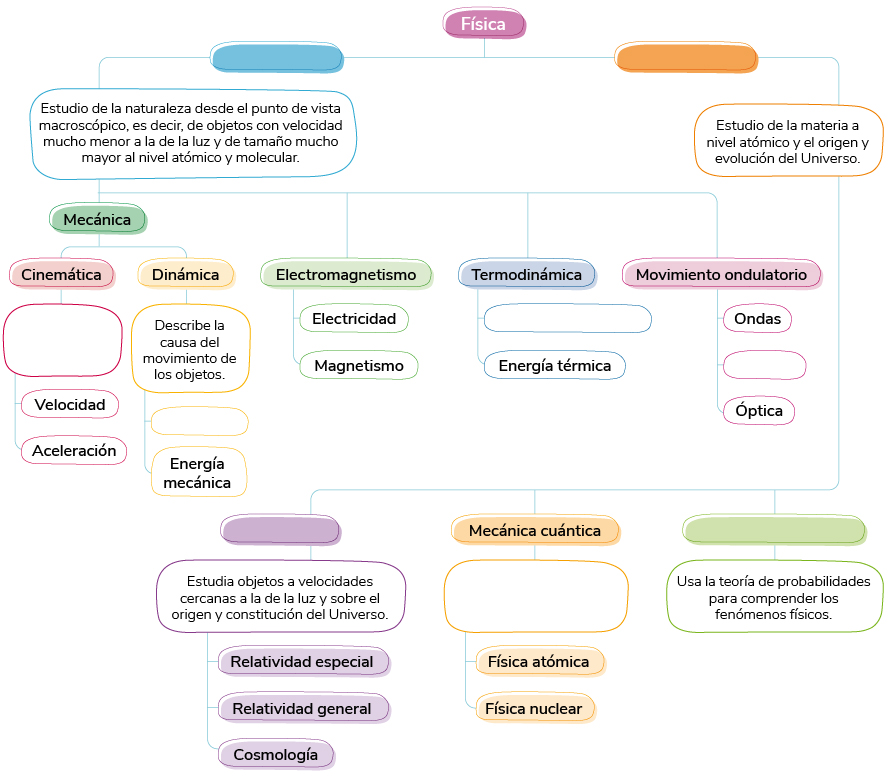
\includegraphics[width=.95\textwidth]{../images/SIM_FI2_SB_U1_P28_IMG01.jpg}
          \end{center}
     }

     \questionboxed[5]{Relaciona las magnitudes físicas fundamentales con su unidad de medida en el Sistema Internacional.

          \begin{multicols}{2}
               \begin{parts}\raggedleft
                    \part Longitud              \fillin[E][0.2in]
                    \part Temperatura           \fillin[B][0.2in]
                    \part Cantidad de sustancia \fillin[G][0.2in]
                    \part Corriente eléctrica   \fillin[D][0.2in]
                    \part Intensidad luminosa   \fillin[F][0.2in]
                    \part Tiempo                \fillin[A][0.2in]
                    \part Masa                  \fillin[C][0.2in]
               \end{parts}

               \columnbreak

               \begin{choices}
                    \choice Segundo
                    \choice Kelvin
                    \choice Kilogramo
                    \choice ampere
                    \choice Metro
                    \choice candela
                    \choice mol
               \end{choices}
          \end{multicols}
     }

     \questionboxed[5]{Señala si son \textit{verdaderas} o \textit{falsas} las siguientes frases:

          \begin{multicols}{2}
               \begin{parts}
                    \part Las unidades derivadas resultan de combinar dos o más unidades fundamentales.

                    \begin{oneparchoices}
                         \choice Verdadero \CorrectChoice Falso
                    \end{oneparchoices}

                    \part Los grados Celsius son una unidad fundamental.

                    \begin{oneparchoices}
                         \CorrectChoice Verdadero \choice Falso
                    \end{oneparchoices}

                    \part Para medir la velocidad se combinan unidades de distancia y de tiempo.

                    \begin{oneparchoices}
                         \choice Verdadero \CorrectChoice Falso
                    \end{oneparchoices}

                    \part El área combina tres veces las unidades de longitud, como los metros cúbicos.

                    \begin{oneparchoices}
                         \CorrectChoice Verdadero \choice Falso
                    \end{oneparchoices}

                    \part Los newtons son una unidad derivada.

                    \begin{oneparchoices}
                         \CorrectChoice Verdadero \choice Falso
                    \end{oneparchoices}

                    \columnbreak

                    \part El milímetro es un múltiplo del metro

                    \begin{oneparchoices}
                         \CorrectChoice Verdadero \choice Falso
                    \end{oneparchoices}

                    \part El kilogramo es un múltiplo del gramo.

                    \begin{oneparchoices}
                         \CorrectChoice Verdadero \choice Falso
                    \end{oneparchoices}

                    \part Los múltiplos del segundo se utilizan para medir tiempos muy pequeños.

                    \begin{oneparchoices}
                         \CorrectChoice Verdadero \choice Falso
                    \end{oneparchoices}

                    \part Los múltiplos del metro se utilizan para medir distancias y longitudes muy grandes.

                    \begin{oneparchoices}
                         \CorrectChoice Verdadero \choice Falso
                    \end{oneparchoices}
               \end{parts}
          \end{multicols}

     }

     \questionboxed[5]{Relaciona los elementos.
          \begin{multicols}{2}
               \begin{parts}\raggedleft\footnotesize
                    \part Número $50 000$ en notación científica.                                                                                           \fillin[][0.2in]
                    \part Número $0.0000032$ en notación científica.                                                                                        \fillin[][0.2in]
                    \part En notación científica es el número $610 000 000 000$.                                                                            \fillin[][0.2in]
                    \part En notación decimal es el número $7.8 \times 10^{-4}$.                                                                            \fillin[][0.2in]
                    \part Notación decimal del número $9.5 \times 108$.                                                                                     \fillin[][0.2in]
                    \part La masa de una ballena azul es de 150 000 kg. ¿Cuál es el valor en notación científica?                                           \fillin[][0.2in]
                    \part El tamaño de un átomo es una diezmilmillonésima de metro, ¿cómo se escribe este número en notación científica?                    \fillin[][0.2in]
                    \part El diámetro de un cabello es de 80 micrómetros. ¿Cuál es este número con notación científica y en metros?                         \fillin[][0.2in]
                    \part La  masa del Sol es $1.989 \times 1030$ kg, si lo escribieras en notación decimal, ¿cuántos ceros tendrías que agregar al número? \fillin[][0.2in]
                    \part La distancia de la Tierra a Neptuno es de 4345 millones de km, ¿cuál es su número con notación científica y en centímetros?       \fillin[][0.2in]
                    \part ¿Cuántos segundos tarda la Tierra en completar una rotación sobre su eje?                                                         \fillin[][0.2in]
                    \part Neptuno tarda 165 años en completar una vuelta alrededor del Sol, ¿a cuántos minutos equivalen, escrito en notación científica?   \fillin[][0.2in]
                    \part La temperatura de la superficie del Sol es de 5772 K, ¿a cuántos mK equivalen?                                                    \fillin[][0.2in]
                    \part La masa de la Tierra es $5.972 \times 10^{24}$ kg. Si la escribieras en notación decimal, ¿cuántos ceros tienes que agregar?      \fillin[][0.2in]
                    \part La masa promedio de una mosca es de 14 mg, ¿cuál es su valor en gramos?.                                                          \fillin[][0.2in]
               \end{parts}

               \columnbreak

               \begin{choices}
                    \choice $5.772  \times 10^6$ mK
                    \choice $10^{-10}$ m
                    \choice $8 \times 10^{-5}$ m
                    \choice $950 000 000$
                    \choice $8.64 \times 10^4$ s
                    \choice $27$
                    \choice $6.1 \times 10^{11}$
                    \choice $0.00078$
                    \choice $0.014$ g
                    \choice $5 \times 10^4$
                    \choice $21$
                    \choice $4.345 \times 10^{14}$ cm
                    \choice $1.5 \times 10^5$ kg
                    \choice $8.672 \times 10^7$ min
                    \choice $3.2 \times 10^{-6}$
               \end{choices}
          \end{multicols}
     }

     \questionboxed[5]{Señala si son \textit{verdaderas} o \textit{falsas} las siguientes frases:
          \begin{multicols}{2}
               \begin{parts}\footnotesize%
                    \part El conocimiento empírico se obtiene a través del método científico y la experimentación controlada.

                    \begin{oneparchoices}
                         \choice Verdadero \CorrectChoice Falso
                    \end{oneparchoices}

                    \part El conocimiento empírico es subjetivo y puede variar entre diferentes individuos.

                    \begin{oneparchoices}
                         \CorrectChoice Verdadero \choice Falso
                    \end{oneparchoices}

                    \part El conocimiento empírico usa el razonamiento lógico.

                    \begin{oneparchoices}
                         \choice Verdadero \CorrectChoice Falso
                    \end{oneparchoices}

                    \part El conocimiento empírico puede estar sujeto a preferencias personales y limitaciones sensoriales.

                    \begin{oneparchoices}
                         \CorrectChoice Verdadero \choice Falso
                    \end{oneparchoices}

                    \part El conocimiento empírico siempre es preciso y objetivo.

                    \begin{oneparchoices}
                         \choice Verdadero \CorrectChoice Falso
                    \end{oneparchoices}

                    \part La base del conocimiento empírico se basa en las experiencias del individuo.

                    \begin{oneparchoices}
                         \CorrectChoice Verdadero \choice Falso
                    \end{oneparchoices}

               \end{parts}
          \end{multicols}
     }

     \questionboxed[5]{Elige la respuesta correcta.
          \begin{multicols}{2}
               \begin{parts}
                    \part ¿Qué es la materia?

                    \begin{choices}
                         \choice La capacidad que tiene un objeto para interactuar con otros \choice El producto de la aceleración por la masa \choice Todo lo que ocupa un lugar en el espacio \choice Todo lo que se puede detectar
                    \end{choices}

                    \part Son propiedades de la materia:

                    \begin{choices}
                         \choice aceleración y fuerza.  \choice distintos medios de propagación.  \choice emoción y sueño.  \choice forma, volumen, masa y compresibilidad.
                    \end{choices}

                    \part La materia \dots

                    \begin{choices}
                         \choice no se puede medir.  \choice es detectable con distintos medios.  \choice no se puede observar.  \choice no ocupa un lugar en el espacio.
                    \end{choices}

                    \columnbreak

                    \part Son materiales que permiten la conducción de calor y electricidad.

                    \begin{choices}
                         \choice Materiales inorgánicos  \choice Materiales metálicos  \choice Materiales tóxicos  \choice Materiales refractarios
                    \end{choices}


                    \part Son materiales derivados del petróleo y pueden ser moldeados para lograr distintos objetos.

                    \begin{choices}
                         \choice Materiales refractarios  \choice Materiales plásticos  \choice Materiales textiles  \choice Materiales metálicos.
                    \end{choices}


               \end{parts}
          \end{multicols}
     }

     \questionboxed[5]{Elige la respuesta correcta.
          \begin{multicols}{2}
               \begin{parts}
                    \part  Es todo aquello que ocupa un lugar en espacio.

                    \begin{choices}
                         \choice Masa  \choice Densidad  \choice Volumen  \CorrectChoice Materia
                    \end{choices}

                    \part Es el espacio que ocupa un objeto.

                    \begin{choices}
                         \choice Masa  \choice Densidad  \CorrectChoice Volumen  \choice Materia
                    \end{choices}

                    \part Es la cantidad de materia que posee un cuerpo.

                    \begin{choices}
                         \CorrectChoice Masa  \choice Densidad  \choice Volumen  \choice Materia
                    \end{choices}
               \end{parts}
          \end{multicols}
     }

     \questionboxed[5]{Señala si son \textit{verdaderas} o \textit{falsas} las siguientes frases:

          \begin{multicols}{2}
               \begin{parts}
                    \part Los electrones son partículas tan pequeñas que no es posible observarlas a simple vista, pero podemos saber de ellas a través de fenómenos como la electricidad, los espectros luminosos y el magnetismo.

                    \begin{oneparchoices}
                         \CorrectChoice Verdadero \choice Falso
                    \end{oneparchoices}

                    \part Los electrones son partículas de carga negativa cubiertas por una nube de carga positiva; la magnitud de ambas cargas es igual, por lo que son eléctricamente neutros.

                    \begin{oneparchoices}
                         \choice Verdadero \CorrectChoice Falso
                    \end{oneparchoices}

                    \part Todos los elementos radiactivos pueden emitir partículas llamadas alfa (carga positiva), beta (carga negativa) y gama (sin carga).

                    \begin{oneparchoices}
                         \CorrectChoice Verdadero \choice Falso
                    \end{oneparchoices}

                    \part En su experimento con partículas alfa, Rutherford encontró que algunas de éstas rebotaban después de chocar con la lámina metálica, por lo que concluyó que colisionaban con obstáculos de carga positiva.

                    \begin{oneparchoices}
                         \CorrectChoice Verdadero \choice Falso
                    \end{oneparchoices}

                    \part Todos los elementos emiten partículas alfa, que poseen carga positiva; beta, que tienen carga negativa; y rayos gama, que no tienen carga eléctrica.

                    \begin{oneparchoices}
                         \choice Verdadero \CorrectChoice Falso
                    \end{oneparchoices}

                    \columnbreak

                    \part El núcleo está formado por protones, que tienen carga positiva, y neutrones, que no poseen carga (es decir, son eléctricamente neutros).

                    \begin{oneparchoices}
                         \CorrectChoice Verdadero \choice Falso
                    \end{oneparchoices}

                    \part Cuando Rutherford colisionó partículas alfa sobre una lámina metálica delgada, encontró que se desviaban muy poco de su trayectoria original, por lo que de inmediato concluyó que el modelo atómico de Thomson era correcto.

                    \begin{oneparchoices}
                         \choice Verdadero \CorrectChoice Falso
                    \end{oneparchoices}

                    \part El modelo de Rutherford no pudo explicar por qué aparecían delgadas líneas oscuras entre las franjas de colores del espectro producido por la luz del Sol; este fenómeno sólo encontraría respuesta con el modelo atómico de Niels Bohr.


                    \begin{oneparchoices}
                         \CorrectChoice Verdadero \choice Falso
                    \end{oneparchoices}

                    \part Si los átomos estuvieran formados sólo por electrones, cualquier objeto estaría cargado negativamente y su electricidad sería evidente.

                    \begin{oneparchoices}
                         \CorrectChoice Verdadero \choice Falso
                    \end{oneparchoices}
               \end{parts}
          \end{multicols}

     }

     \questionboxed[5]{Señala si los siguientes procesos son \textit{físicos} o \textit{químicos}.
          \begin{multicols}{2}
               \begin{parts}
                    \part Romper una hoja de papel.

                    \begin{oneparchoices}
                         \CorrectChoice Físico \choice Químico
                    \end{oneparchoices}

                    \part Digerir y absorber los alimentos.

                    \begin{oneparchoices}
                         \choice Físico \CorrectChoice Químico
                    \end{oneparchoices}

                    \part Derretir una vela.

                    \begin{oneparchoices}
                         \CorrectChoice Físico \choice Químico
                    \end{oneparchoices}

                    \part Encender fuegos artificiales.

                    \begin{oneparchoices}
                         \choice Físico \CorrectChoice Químico
                    \end{oneparchoices}

                    \part Hornear un pastel de vainilla.

                    \begin{oneparchoices}
                         \choice Físico \CorrectChoice Químico
                    \end{oneparchoices}

                    \part Apretar una lata de aluminio.

                    \begin{oneparchoices}
                         \CorrectChoice Físico \choice Químico
                    \end{oneparchoices}

                    \part Derretir un cubo de hielo.

                    \begin{oneparchoices}
                         \CorrectChoice Físico \choice Químico
                    \end{oneparchoices}

                    \part Cocinar un huevo estrellado.

                    \begin{oneparchoices}
                         \choice Físico \CorrectChoice Químico
                    \end{oneparchoices}
               \end{parts}
          \end{multicols}
     }



     \questionboxed[10]{Coloca los conceptos en el lugar que les corresponda en la imagen.\\

          \begin{center}
               \wordpill{Modelo atómico del ``panqué con pasas''}
               \wordpill{El descubrimiento del electrón}
               \wordpill{Ernest Rutherford}
               \wordpill{El descubrimiento del núcleo atómico}
               \wordpill{Neutrones}
               \wordpill{Niels Bohr}
               \wordpill{Modelo Cuántico del átomo}
               \wordpill{Explicar los espectros luminosos}
               \wordpill{Descubrir el átomo de hidrógeno}
               \vspace*{1em}
               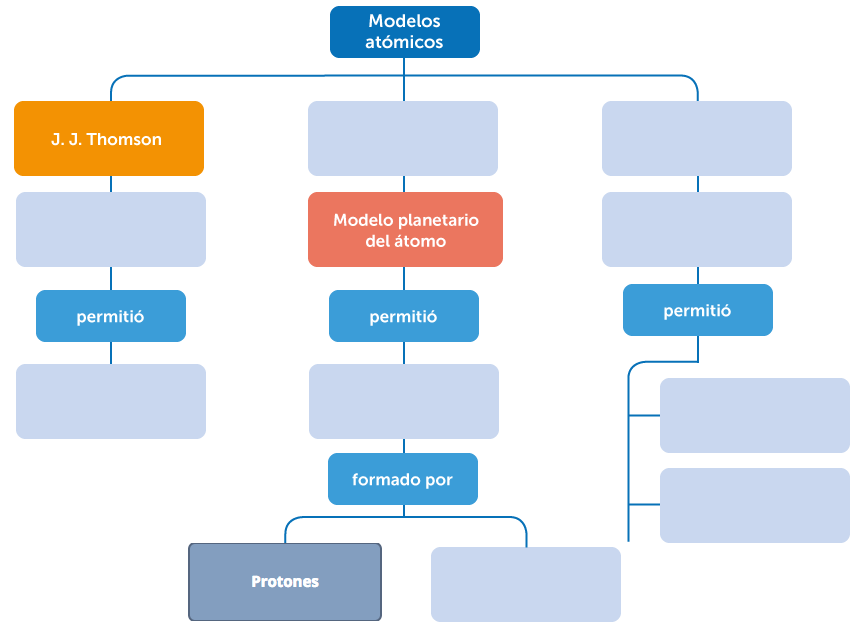
\includegraphics[width=.9\textwidth]{../images/SINFI_U2_AC65_IMGS1.png}
          \end{center}
     }

     \questionboxed[5]{Ordena los pasos del método científico.

          \begin{parts}\footnotesize%
               \part \fillin[5][0.2in] Análisis de resultados
               \part \fillin[4][0.2in] Experimentación
               \part \fillin[7][0.2in] Comunicación de resultados
               \part \fillin[9][0.2in] Teoría científica
               \part \fillin[1][0.2in] Observación
               \part \fillin[8][0.2in] Ley científica
               \part \fillin[2][0.2in] Planteamiento del problema
               \part \fillin[6][0.2in] Verificación de la hipótesis
               \part \fillin[3][0.2in] Hipótesis
          \end{parts}
     }

     \questionboxed[5]{Elige la respuesta para cada pregunta.
          \begin{multicols}{2}
               \begin{parts}
                    \part Un corresponsal de noticias informa que las altas temperaturas en California, Estados Unidos, alcanzaron 113 °F. ¿Cuál es la temperatura equivalente en grados centígrados?

                    \begin{oneparchoices}
                         \CorrectChoice 45 °C \choice 55 °C
                    \end{oneparchoices}

                    \part José observa el informe del clima durante un viaje de negocios en Dublín (Irlanda). El conductor de noticias asegura que la temperatura se elevará de los 64.4 °F actuales a 102.2 °F. ¿Cuál es el incremento de temperatura correspondiente en la escala Celsius?

                    \begin{oneparchoices}
                         \CorrectChoice 21 °C \choice 37.8 °C
                    \end{oneparchoices}

                    \part Pedro se siente mal y decide ir al médico, éste le informa que su temperatura corporal es de 313.15 K. Pedro sabe que una persona tiene fiebre cuando su temperatura es superior a 37 °C. ¿Cuál es el estado de salud de Pedro?

                    \begin{oneparchoices}
                         \CorrectChoice Pedro tiene fiebre \choice Pedro no tiene fiebre
                    \end{oneparchoices}

                    \part Mónica cocinará un pavo en Navidad y desea que su familia realmente lo disfrute, por lo que se prepara estudiando un recetario de cocina profesional. En él encuentra que debe precalentar el horno a 325 °F, pero su horno utiliza la escala Celsius. ¿Cuál es la temperatura equivalente?

                    \begin{oneparchoices}
                         \CorrectChoice 100 °C \choice 162.7 °C
                    \end{oneparchoices}

                    \part De compras en un centro comercial, Francisco lee en la etiqueta de una lata de atún: “Mantener por debajo de 296.15 K. ¿Cuál es la temperatura correspondiente en la escala Celsius?

                    \begin{oneparchoices}
                         \CorrectChoice 23 °C \choice 47 °C
                    \end{oneparchoices}


                    \part Mexicali, capital de Baja California, es la ciudad más calurosa de México. Debido a su ubicación de tipo desierto interior, las temperaturas alcanzan 40 °C. ¿A qué temperatura equivale esto en la escala Fahrenheit?

                    \begin{oneparchoices}
                         \CorrectChoice 72 °F \choice 104 °F
                    \end{oneparchoices}

                    \part El cuerpo humano resiste mejor los descensos de temperatura que los aumentos en la misma. Un descenso significativo de temperatura sólo provoca una lentificación de las funciones celulares, mientras que un aumento de la misma magnitud provocaría la pérdida definitiva de tales funciones. La temperatura máxima que puede soportar el cuerpo humano es 316.15 K. ¿A qué temperatura equivale en la escala Celsius y Fahrenheit?

                    \begin{oneparchoices}
                         \choice 109,4 °C y 43 °F \CorrectChoice 43 °C y 109.4 °F
                    \end{oneparchoices}

                    \part El 10 de agosto del 2010, un grupo de investigadores registró en la Antártida la temperatura más baja del planeta: 93 °C bajo cero. ¿Cuál es la temperatura correspondiente en la escala de temperatura absoluta?

                    \begin{oneparchoices}
                         \CorrectChoice 180.15 K \choice 366.15 K
                    \end{oneparchoices}

                    \part Venus no es el planeta más cercano al Sol, pero sí el más caliente, pues posee una atmósfera muy densa que impide que el calor proveniente del Sol escape del planeta (efecto invernadero). Alcanza temperaturas de hasta 864 °F. ¿Cuál es la temperatura correspondiente en la escala Celsius?

                    \begin{oneparchoices}
                         \CorrectChoice 462.22 °C \choice 1587.2 °C
                    \end{oneparchoices}

                    \part Rubén colocó un vaso con agua en el refrigerador y lo dejó ahí hasta que el agua sufrió un descenso de temperatura de 20.3 °C. ¿Cuál es el cambio de temperatura correspondiente en K?

                    \begin{oneparchoices}
                         \choice 20.3 K \CorrectChoice 293.45 K
                    \end{oneparchoices}

                    \part Según la agencia científica de Naciones Unidas, la temperatura promedio en la superficie de la Tierra y de los océanos fue la más alta en el periodo de enero a octubre de 2014, al alcanzar 14.78 °C. ¿Cuál es la temperatura correspondiente en grados Fahrenheit?

                    \begin{oneparchoices}
                         \choice 26.604 °F \CorrectChoice  58.604 °F
                    \end{oneparchoices}

                    \part El punto de fusión del oro es 1 064 °C y la plata se funde a 1 234.93 K. ¿Cuál de los dos tiene una temperatura de fusión más elevada?

                    \begin{oneparchoices}
                         \CorrectChoice El oro \choice La plata
                    \end{oneparchoices}

               \end{parts}
          \end{multicols}

     }

     \questionboxed[5]{Elige la respuesta correcta
          \begin{multicols}{2}
               \begin{parts}
                    \part Indica con claridad el problema que se quiere resolver. Delimita y especifica el objeto de su investigación.

                    \begin{choices}
                         \choice Experimentación
                         \CorrectChoice Planteamiento del problema
                         \choice Ley científica
                         \choice Comunicación de resultados
                    \end{choices}

                    \part Se trata de demostrar si la hipótesis es o no correcta mediante un experimento controlado.

                    \begin{choices}
                         \choice Hipótesis
                         \choice Observación
                         \choice Teoría científica
                         \CorrectChoice Experimentación
                    \end{choices}

                    \part Indica la regularidad que existe en un fenómeno, entre sus causas y sus efectos, normalmente se expresa de manera matemática.

                    \begin{choices}
                         \choice Hipótesis
                         \CorrectChoice Ley científica
                         \choice Teoría científica
                         \choice Experimentación
                    \end{choices}

                    \part Si no se comprueba la hipótesis, se plantea una nueva, considerando los datos y la información obtenida en el experimento.

                    \begin{choices}
                         \CorrectChoice Verificación de la hipótesis
                         \choice Análisis de resultados
                         \choice Teoría científica
                         \choice Comunicación de resultados
                    \end{choices}

                    \columnbreak

                    \part El científico observa la realidad que le rodea, aísla el fenómeno que le interesa e identifica las variables que intervienen.

                    \begin{choices}
                         \choice Hipótesis
                         \CorrectChoice Observación
                         \choice Teoría científica
                         \choice Verificación de la hipótesis
                    \end{choices}

                    \part Propuesta de una posible explicación del fenómeno.

                    \begin{choices}
                         \CorrectChoice Hipótesis
                         \choice Observación
                         \choice Teoría científica
                         \choice Experimentación
                    \end{choices}

                    \part La hipótesis se confirma o se rechaza analizando los datos y la información obtenida en los experimentos.

                    \begin{choices}
                         \choice Ley científica
                         \choice Observación
                         \CorrectChoice Análisis de resultados
                         \choice Experimentación
                    \end{choices}

                    \part El científico comparte los resultados de su investigación a la comunidad científica mediante tesis, artículos científicos o congresos.

                    \begin{choices}
                         \choice Ley científica
                         \choice Análisis de resultados
                         \choice Teoría científica
                         \CorrectChoice Comunicación de resultados
                    \end{choices}

                    \part Explicación de un fenómeno a partir de leyes científicas.

                    \begin{choices}
                         \CorrectChoice Teoría científica
                         \choice Ley científica
                         \choice Análisis de resultados
                         \choice Comunicación de resultados
                    \end{choices}
               \end{parts}
          \end{multicols}
     }
\end{questions}
\end{document}